\chapter{Моделювання Кризових Явищ.}

\textbf{Кризове явище} - це різка або суттєва зміна стану системи, яка призводить до негативних наслідків і може порушити її нормальне функціонування. З точки зору інтелектуального аналізу даних кризові явища розглядаються як події, що можуть бути виявлені або передбачені на основі аналізу історичних даних.

Серед прикладів кризових явищ можна визначити фінансові кризи та економічні спади, епідемії, техногенні аварії, природні катастрофи та масові кібератаки. Основною метою аналізу є своєчасне виявлення ознак наближення кризи та прогнозування її розвитку.

Передбачення криз дозволяє завчасно приймати управлінські рішення та мінімізувати можливі збитки. Завдяки прогнозуваннюю можна своєчасно виявляти ризики та планувати заходи врегулювання.

\section{Передбачення фінансових криз.}

Для прогнозування економічних криз можна використовувати великі обсяги фінансових даних. Зокрема, для цього добре підійдуть ціни акцій та фондові індекси, валютні курси та процентні ставки, рівні безробіття та інфляції, ВВП та кредитна активність, та багато інших. Поєднання різних джерел даних дозволяє підвищити точність прогнозування.

У прогнозуванні фінансових криз використовуються різні задачі машинного навчання.

Найпоширенішими є:

\begin{itemize}
\item класифікація — визначення, чи існує ризик виникнення кризи;
\item регресія — прогнозування числових економічних показників;
\item аналіз часових рядів — прогнозування майбутніх значень економічних індикаторів;
\item кластеризація — виявлення груп країн або компаній із подібною фінансовою поведінкою;
\item виявлення аномалій — пошук нетипових змін, що можуть передувати кризі.
\end{itemize}

Кожна з цих задач допомагає досліджувати кризові процеси з різних сторін. Для прогнозування криз використовують як класичні статистичні методи, так і сучасні алгоритми машинного навчання.

Методи машинного навчання мають низку переваг порівняно з традиційними економічними моделями. Вони дозволяють працювати з великими обсягами даних, знаходити складні нелінійні залежності та приховані закономірності в фінансових даних.

В той же час, прогнозування фінансових криз є складною задачею через особливості економічних процесів. Кількість історичних криз достатньо невелика - у нас просто замало даних. Фінансові дані часто містять велику кількість шуму, а моделі що вчаться на цих даних підпадають під ризик перенавчання. Крім того, на економічні процеси можуть суттєво впливати політичні рішення, міжнародні конфлікти та інші непередбачувані події. 

Будь-яка модель машинного навчання навчається на наявних даних. Якщо фінансові дані є неповними, неточними або містять помилки, модель також формуватиме неправильні прогнози.

Завантажемо дані з ринку $S\&P$ 500 цінних паперів, дані про дохідність облігацій (як економічний індикатор), та об'єднаємо ці датасети за датами.

\begin{lstlisting}
import numpy as np
import pandas as pd
import yfinance as yf
import matplotlib.pyplot as plt
import seaborn as sns
from sklearn.model_selection import train_test_split
from sklearn.ensemble import RandomForestClassifier
from sklearn.metrics import classification_report, confusion_matrix

sp500_data = yf.download('^GSPC', start='2000-01-01', end='2023-01-01')

print(sp500_data.head(10))
sp500_data['Return'] = sp500_data['Close'].pct_change()  # Calculate daily returns

bond_yield_data = yf.download('^TNX', start='2000-01-01', end='2023-01-01') 
bond_yield_data['Yield'] = bond_yield_data['Close']

data = sp500_data[['Return']].merge(bond_yield_data[['Yield']], left_index=True, right_index=True)
data.dropna(inplace=True)  

sp500_data[:10]
\end{lstlisting}

Результат:

\begin{console}
Price             Close         High          Low         Open      Volume
Ticker            ^GSPC        ^GSPC        ^GSPC        ^GSPC       ^GSPC
Date                                                                      
2000-01-03  1455.219971  1478.000000  1438.359985  1469.250000   931800000
2000-01-04  1399.420044  1455.219971  1397.430054  1455.219971  1009000000
2000-01-05  1402.109985  1413.270020  1377.680054  1399.420044  1085500000
2000-01-06  1403.449951  1411.900024  1392.099976  1402.109985  1092300000
2000-01-07  1441.469971  1441.469971  1400.729980  1403.449951  1225200000
2000-01-10  1457.599976  1464.359985  1441.469971  1441.469971  1064800000
2000-01-11  1438.560059  1458.660034  1434.420044  1457.599976  1014000000
2000-01-12  1432.250000  1442.599976  1427.079956  1438.560059   974600000
2000-01-13  1449.680054  1454.199951  1432.250000  1432.250000  1030400000
2000-01-14  1465.150024  1473.000000  1449.680054  1449.680054  1085900000
[*********************100%***********************]  1 of 1 completed
\end{console}

Нам потрібно визначити, що таке фінансова криза. Загальноприйнятий підхід полягає у виділенні періодів екстремального спаду на ринку, коли прибутковість фондового ринку значно падає за короткий проміжок часу.

Визначимо кризову ситуацію, якщо прибутковість опуститься нижче певного порогового значення (наприклад, -5 $\%$ за один день). Перевіримо розподіл кризових моментів.

\begin{lstlisting}
data['Crisis'] = (data['Return'] < -0.05).astype(int)

print(data['Crisis'].value_counts())

plt.figure(figsize=(12, 6))
plt.subplot(2, 1, 1)
plt.plot(data.index, data['Return'], label='S&P 500 Returns')
plt.axhline(y=-0.05, color='r', linestyle='--', label='Crisis Threshold (-5%)')
plt.legend()
plt.title('S&P 500 Daily Returns')

plt.subplot(2, 1, 2)
plt.plot(data.index, data['Yield'], label='10-Year Treasury Yield')
plt.title('10-Year Treasury Yield')
plt.tight_layout()
plt.show()
\end{lstlisting}

Результат:

\begin{console}
Crisis
0    5761
1      19
Name: count, dtype: int64
\end{console}

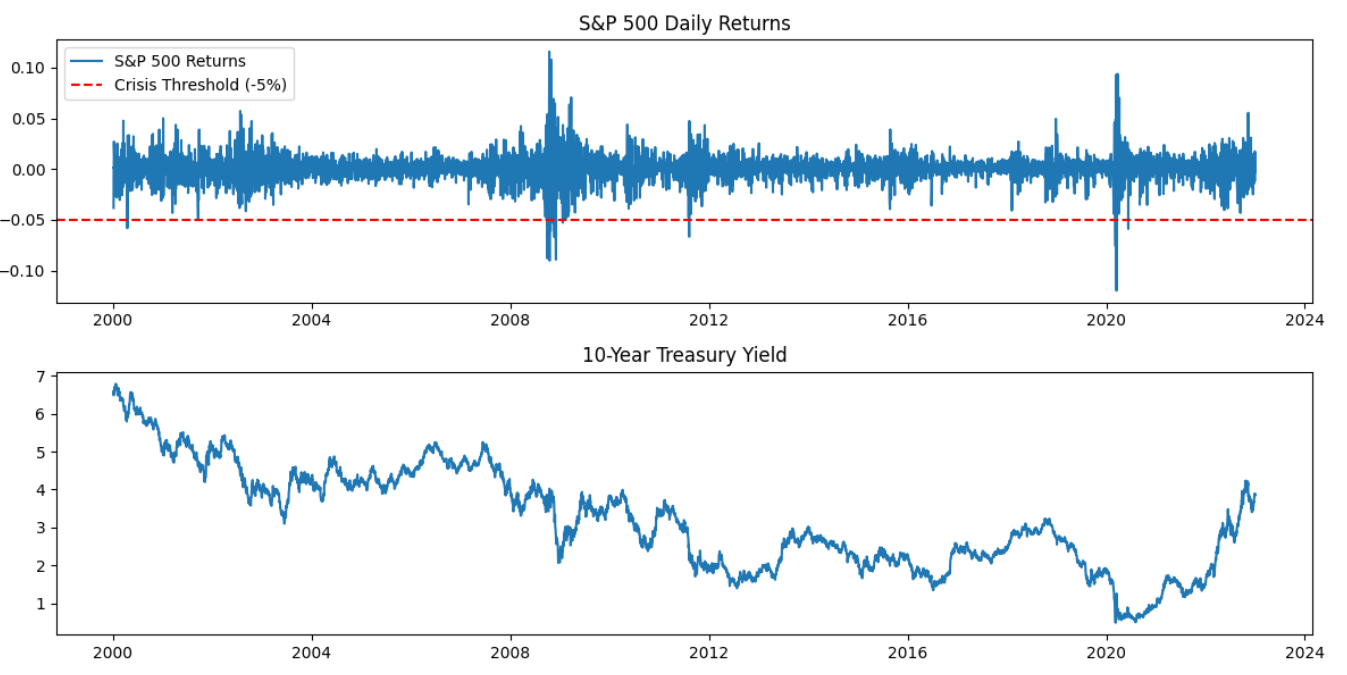
\includegraphics[scale=0.5]{img/209-1}

Ми розділимо дані на навчальні та тестові набори, щоб оцінити ефективність нашої моделі. 

Визначаємо характеристики (економічні показники) та ціль (мітку «Криза»), та розділяємо дані на тестові та тренувальні:

\begin{lstlisting}
X = data[['Return', 'Yield']]
y = data['Crisis']

X_train, X_test, y_train, y_test = train_test_split(X, y, test_size=0.2, shuffle=False)
\end{lstlisting}

Ми будемо використовувати RandomForestClassifier для моделювання взаємозв'язку між економічними показниками та кризовими подіями.

\begin{lstlisting}
model = RandomForestClassifier(n_estimators=100, random_state=42)
model.fit(X_train, y_train)
\end{lstlisting}

Результат:

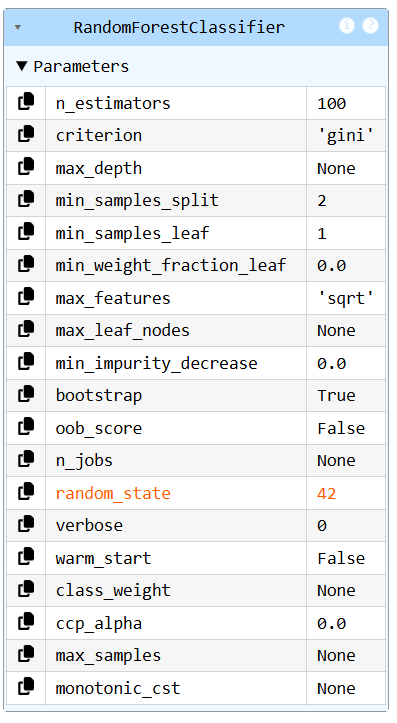
\includegraphics[scale=0.5]{img/209-2}

Після навчання моделі ми оцінюємо її ефективність за допомогою матриці плутанини та звіту про класифікацію.

\begin{lstlisting}
y_pred = model.predict(X_test)

print(confusion_matrix(y_test, y_pred))
print(classification_report(y_test, y_pred))

plt.figure(figsize=(12, 6))
plt.plot(y_test.index, y_test.values, label='Actual Crisis Events', color='r', linestyle='--')
plt.plot(y_test.index, y_pred, label='Predicted Crisis Events', color='g')
plt.title('Actual vs Predicted Financial Crises')
plt.legend()
plt.show()
\end{lstlisting}

Результат:

\begin{console}
[[1151    0]
 [   0    5]]
              precision    recall  f1-score   support

           0       1.00      1.00      1.00      1151
           1       1.00      1.00      1.00         5

    accuracy                           1.00      1156
   macro avg       1.00      1.00      1.00      1156
weighted avg       1.00      1.00      1.00      1156
\end{console}

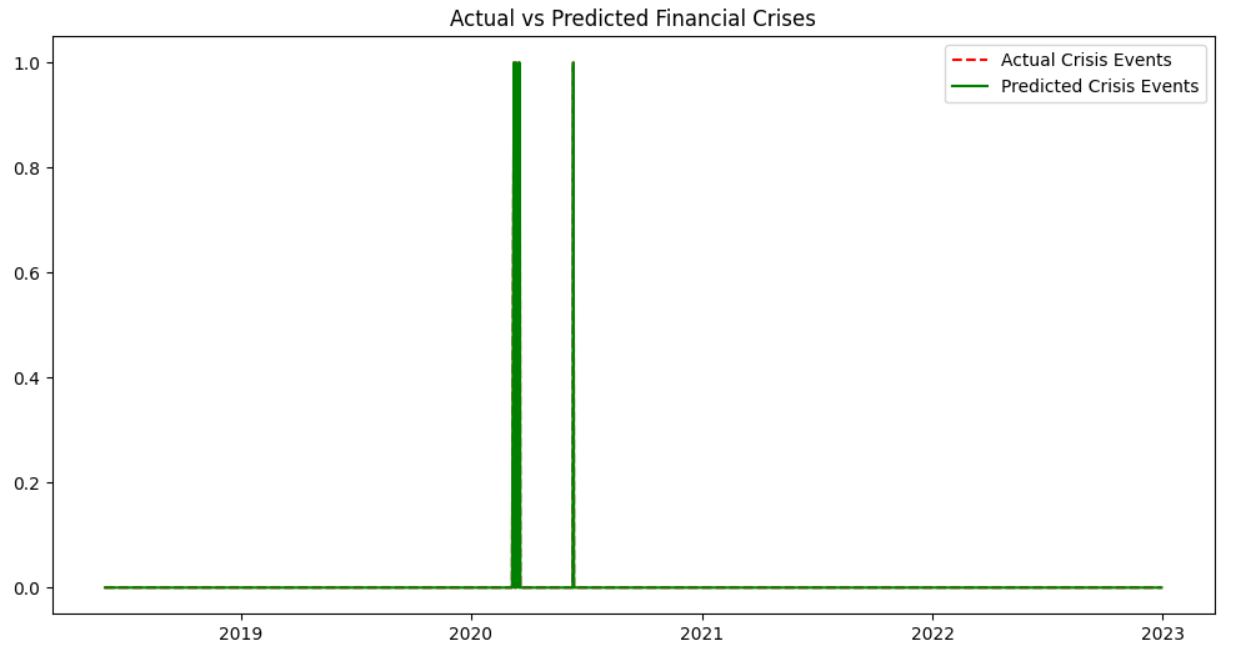
\includegraphics[scale=0.5]{img/209-3}




\section{Моделювання розповсюдження епідемій.}

\textbf{Епідеміологічне моделювання} - це побудова математичних або комп'ютерних моделей, які описують поширення інфекційних захворювань серед населення. Такі моделі дозволяють досліджувати механізми передачі інфекції, оцінювати швидкість її поширення, прогнозувати кількість хворих у майбутньому та аналізувати ефективність різних протиепідемічних заходів. Епідеміологічне моделювання широко застосовується в медицині, громадському здоров'ї та державному управлінні для прийняття обґрунтованих рішень під час спалахів інфекційних хвороб.


\textbf{SIR-модель} — це одна з найвідоміших математичних моделей для опису поширення інфекційних захворювань у популяції. Вона дозволяє зрозуміти, як хвороба поширюється, коли досягає піку та за яких умов епідемія згасає. Модель була запропонована Кермаком та МакКендріком у 1927 році і досі є основою епідеміологічного моделювання.

SIR — це абревіатура від трьох станів, у яких може знаходитися кожна людина в популяції:

\begin{itemize}
\item S (Susceptible) — сприйнятливі: Люди, які ще не хворіють, але можуть заразитися.

\item I (Infectious) — інфіковані:    Люди, які хворіють і здатні передавати інфекцію іншим.

\item R (Recovered/Removed) — одужалі (або видалені): Люди, які або одужали й отримали імунітет, або були ізольовані, або померли (тобто не взаємодіють із іншими).
\end{itemize}

Популяція вважається закритою, тобто:

$$
N = S(t) + I(t) + R(t) = const
$$

Система диференціальних рівнянь: SIR-модель описується трьома рівняннями:

$$
\frac{dS(t)}{dt} = -\beta \frac{S(t) *I(t)}{N}
$$

$$
\frac{dI}{dt} = \beta \frac{S I}{N} - \gamma I
$$

$$
\frac{dR}{dt} = \gamma I
$$

тут $\beta$ (бета) - коефіцієнт інфікування - показує, як часто відбуваються контакти та з якою ймовірністю вони ведуть до зараження; $\gamma$ (гама) - коефіцієнт одужання - це швидкість переходу з $I \rightarrow R$. Якщо середня тривалість хвороби — $D$ днів, то:
  $$
  \gamma \approx \frac{1}{D}
  $$

Коефіцієнт зараження $\beta$ визначає, наскільки швидко інфекція поширюється серед населення. Якщо його значення велике, кожен інфікований заражає більше людей, тому кількість хворих швидко зростає, а пік епідемії настає раніше. Якщо ж значення коефіцієнта невелике, поширення інфекції відбувається повільніше, а епідемічна крива стає більш пологою.

Коефіцієнт одужання $\gamma$ визначає, як швидко інфіковані люди перестають бути джерелом зараження. Чим більшим є цей коефіцієнт, тим швидше люди одужують, а отже, тим менше часу вони можуть передавати інфекцію іншим. У результаті зменшується кількість одночасно хворих людей і скорочується тривалість епідемії.

Базове репродуктивне число $R_0$ - найважливіший параметр епідемії:

$$
R_0 = \frac{\beta}{\gamma}
$$

Якщо $R_0 > 1$ — хвороба поширюється, епідемія. Якщо $R_0 < 1$ — хвороба згасає.

Інтуїтивно це означає, скільки людей у середньому заразить один хворий у незахищеній популяції.

Параметри моделі безпосередньо визначають форму епідемічної кривої. Збільшення коефіцієнта зараження призводить до швидкого зростання кількості інфікованих і більш високого піку захворюваності. Збільшення коефіцієнта одужання, навпаки, зменшує висоту піку та прискорює завершення епідемії. Комбінація цих параметрів дозволяє моделювати різні сценарії розвитку захворювання та оцінювати можливий вплив карантинних обмежень або вакцинації.

Динаміка епідемії, типовий перебіг для SIR: на початку багато S та мало I, інфекція швидко росте. Максимальне значення I досягається доволі швидко, потім воно спадає. З часом S зменшується, тому інфікування сповільнюється. Коли кількість сприйнятливих падає нижче певного порогу, хвиля епідемії природно згасає. Збільшується група R — тих, хто набув імунітету.

Інтерпретація кривих: на графіку зазвичай видно, як S(t) плавно зменшується; I(t) різко зростає, досягає піку, потім спадає, та R(t) зростає та стабілізується.

Пік I(t) залежить від параметрів $\beta$ та $\gamma$ — і саме його намагаються "сплющити" карантинними заходами.

Спочатку імпортуємо необхідні для роботи модулі та задамо параметри моделі: чисельність населення N, початкове число інфікованих I0, початкове число виздоровівших/вилучених R0, початкове число тих, хто може бути зараженим S0, коефіцієнти інфікування та виздоровлення beta та gamma:

\begin{lstlisting}
import numpy as np
from scipy.integrate import odeint
import matplotlib.pyplot as plt

N = 1000         
I0 = 1         
R0 = 0           
S0 = N - I0 - R0 
beta = 0.5    
gamma = 0.1    
\end{lstlisting}

Визначимо часовий проміжок:

\begin{lstlisting}
t = np.linspace(0, 160, 160)
\end{lstlisting}

Систему диференціальних рівнянь визначимо за допомогою наступного методу: 

\begin{lstlisting}
def sir_model(y, t, N, beta, gamma):
    S, I, R = y
    dSdt = -beta * S * I / N
    dIdt = beta * S * I / N - gamma * I
    dRdt = gamma * I
    return dSdt, dIdt, dRdt
\end{lstlisting}

Зрештою, сама SIR модель рівнянь за часом t:

\begin{lstlisting}
y0 = S0, I0, R0

ret = odeint(sir_model, y0, t, args=(N, beta, gamma))
S, I, R = ret.T
\end{lstlisting}

Повністю разом із побідовую результатів на графіку:


\begin{lstlisting}
import numpy as np
from scipy.integrate import odeint
import matplotlib.pyplot as plt

N = 1000         
I0 = 1         
R0 = 0           
S0 = N - I0 - R0 
beta = 0.5    
gamma = 0.1    

t = np.linspace(0, 160, 160)

def sir_model(y, t, N, beta, gamma):
    S, I, R = y
    dSdt = -beta * S * I / N
    dIdt = beta * S * I / N - gamma * I
    dRdt = gamma * I
    return dSdt, dIdt, dRdt

y0 = S0, I0, R0

ret = odeint(sir_model, y0, t, args=(N, beta, gamma))
S, I, R = ret.T

plt.figure(figsize=(10, 6))
plt.plot(t, S, 'b', label='Susceptible')
plt.plot(t, I, 'r', label='Infected')
plt.plot(t, R, 'g', label='Recovered')
plt.xlabel('Time (days)')
plt.ylabel('Population')
plt.title('COVID-19 Spread Simulation Using SIR Model')
plt.legend()
plt.show()
\end{lstlisting}

Результат:

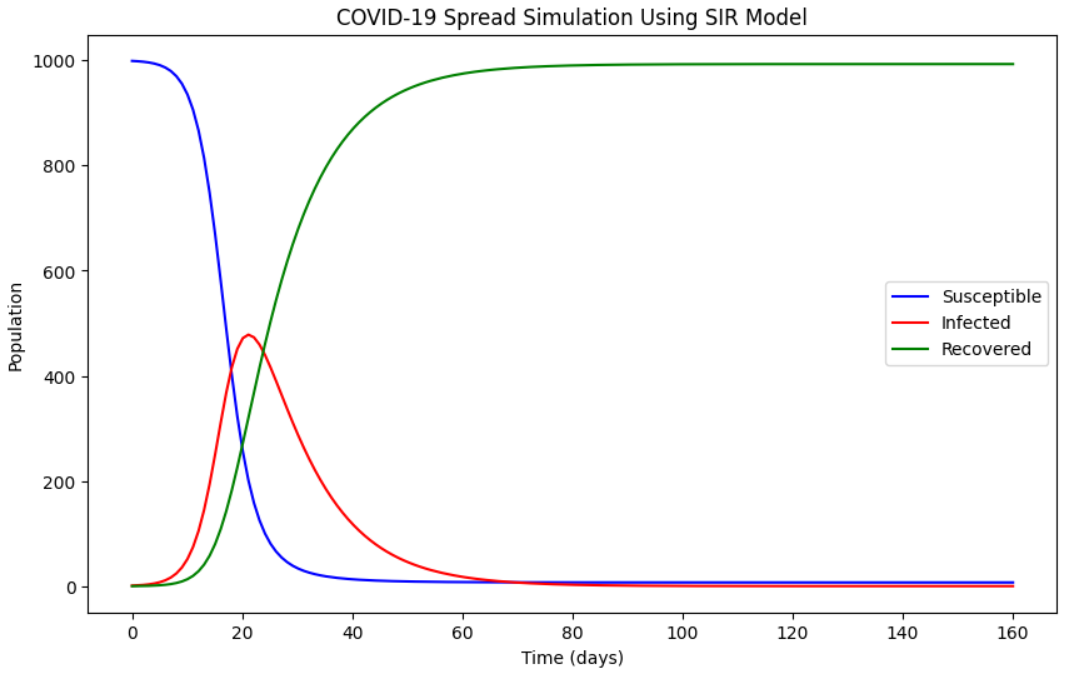
\includegraphics[scale=0.5]{img/209-4}

Класична модель SIR базується на низці спрощувальних припущень. Вона вважає, що всі люди однаково контактують між собою, не враховує вікову структуру населення, географічне розташування, різницю в поведінці людей, повторні зараження та зміну параметрів поширення інфекції з часом. Крім того, модель не враховує вплив вакцинації, мутацій вірусу чи державних обмежувальних заходів, якщо вони не вводяться окремо.

Методи машинного навчання дозволяють враховувати значно більшу кількість факторів, ніж класичні математичні моделі. Вони можуть аналізувати мобільність населення, погодні умови, соціально-економічні показники, статистику вакцинації, дані соціальних мереж та інші джерела інформації. Поєднання моделей SIR із методами машинного навчання дає змогу автоматично оцінювати параметри моделі, підвищувати точність прогнозування та швидше адаптуватися до нових умов розвитку епідемії.

Сучасний розвиток штучного інтелекту значно розширює можливості моделювання кризових явищ. Використання великих даних дозволяє аналізувати інформацію з численних джерел у режимі реального часу, а сучасні алгоритми машинного навчання здатні виявляти складні закономірності, які важко помітити традиційними методами. Особливо перспективними є глибокі нейронні мережі, Transformer-моделі, графові нейронні мережі та генеративний штучний інтелект. У майбутньому очікується поєднання класичних математичних моделей із методами машинного навчання, що забезпечить більш точне прогнозування криз, швидшу адаптацію моделей до нових умов і можливість підтримки прийняття рішень у реальному часі.

\ding{46} \textbf{Питання для самоконтролю.}

\begin{enumerate}
\item Що таке кризове явище з точки зору аналізу даних?
\item Які типи кризових явищ можна моделювати за допомогою методів машинного навчання?
\item Чому прогнозування кризових явищ є важливим завданням інтелектуального аналізу даних?
\item Які дані використовуються для прогнозування фінансових криз?
\item Які економічні показники можуть бути ознаками наближення фінансової кризи?
\item Які задачі машинного навчання застосовуються для прогнозування фінансових криз?
\item Які алгоритми машинного навчання найчастіше використовуються для прогнозування кризових явищ?
\item Які переваги має використання машинного навчання порівняно з традиційними економічними моделями?
\item Які труднощі виникають під час побудови моделей прогнозування фінансових криз?
\item Чому якість даних є критично важливою для прогнозування кризових явищ?
\item Що таке епідеміологічне моделювання?
\item Для чого використовується модель SIR?
\item Які групи населення виділяє модель SIR?
\item Що означає категорія Susceptible (S) у моделі SIR?
\item Що означає категорія Infected (I) у моделі SIR?
\item Що означає категорія Recovered (R) у моделі SIR?
\item Які параметри використовуються в моделі SIR?
\item Як коефіцієнт зараження впливає на поширення епідемії?
\item Як коефіцієнт одужання впливає на перебіг епідемії?
\item Що таке базове репродуктивне число $R_{0}$ і як воно інтерпретується?
\item Як зміна параметрів моделі SIR впливає на форму епідемічної кривої?
\item Які обмеження має класична модель SIR?
\item Як методи машинного навчання можуть доповнювати математичні моделі поширення епідемій?
\item У яких практичних сферах використовуються моделі прогнозування кризових явищ?
\item Які перспективи розвитку моделювання кризових явищ пов'язані зі штучним інтелектом, аналізом великих даних та сучасними методами машинного навчання?
\end{enumerate}